\documentclass[11pt]{article}
\usepackage[hmargin=2cm,vmargin=2cm]{geometry}
\usepackage{natbib}
\usepackage[english]{babel}
\usepackage{graphicx}
\usepackage{amstext}
\usepackage{setspace}
\usepackage{threeparttable}
\usepackage{subfigure}
\usepackage{booktabs}
\usepackage{rotating}
\usepackage{float}
\usepackage{fancybox}
\usepackage{xcolor}
\usepackage{array,color}
\usepackage{dcolumn}
\usepackage[font=small,labelfont=bf]{caption}
\usepackage{longtable}
\usepackage{verbatim}
\usepackage{pdflscape}
\usepackage{amssymb}
\usepackage{lscape}
\usepackage{tabularx}
\usepackage{verbatim}
\usepackage{geometry}
\usepackage{bbold}
\usepackage{apalike}
%\usepackage{hyperref}
\usepackage{mathtools}
\usepackage{amsmath}
\usepackage{color,soul}
\usepackage{bibentry}
\usepackage{pxfonts}
\usepackage{palatino}
\usepackage{authblk}
\usepackage{enumitem}
\usepackage[toc,page]{appendix}
\usepackage{chngcntr}
\usepackage[utf8]{inputenc}
\usepackage{pdflscape}
\setlength{\parindent}{1cm}
\setlength{\parskip}{2mm}
\usepackage{lipsum}




%%%%%%%%%%%%%%%%%%%%%%%%%%%%%%%%%%%%%%%%%%%%%%%%%%%%%%%%%%%%%%
\title{Recreation of Temperature and Decisions: Evidence from 207,000
	Court Cases}
\author{Viktor Reif}
\date{\today}


\begin{document}
	\maketitle
	
	
	%%%%%%%%%%%%%%%%%%%%%%%%%%%%%%%%%%%%%%%%%%%%%%%%%%%%%%%%%%%%%%
	% Abstract
	%%%%%%%%%%%%%%%%%%%%%%%%%%%%%%%%%%%%%%%%%%%%%%%%%%%%%%%%%%%%%%
	\begin{abstract}
		\singlespacing
		\noindent 
		\textit{(note: cursive indicates my comments) 0. Abstract: summarize the key points of the paper.}
		I replicate the main results of the paper "Temperature and Decisions: Evidence from 207,000 Court Cases" by \cite{Heyes.2019} and evaluate the validity of its empirical findings. The paper's underlying specification to model the effect of outdoor temperature on asylum court case outcomes is a panel model including control variables for weather, pollution and case characteristics as well as several fixed effects for entities, time and space dynamics. I find the same effects as Heyes and Saberian. Yet through a more thorough analysis (sampling, specification and data issues) get results that question the validity of the original findings. Using yearly subsamples of the entire dataset (2000-2004) yields temperature effects that are not significantly different from zero for all but one year.
		\newline \noindent \textbf{Keywords:} decision-making; temperature; fixed-effects regression; spatial panel data
	\end{abstract} \newpage

	
	
	%%%%%%%%%%%%%%%%%%%%%%%%%%%%%%%%%%%%%%%%%%%%%%%%%%%%%%%%%%%%%%
	% Section 1: 
	%%%%%%%%%%%%%%%%%%%%%%%%%%%%%%%%%%%%%%%%%%%%%%%%%%%%%%%%%%%%%%
	\section{Introduction}
	\textit{introduce the topic and state the aim of your work, stating clearly the research questions and the methodology used, give a brief overview of the results and the limitations of your analysis.}
	\newline This paper examines the robustness of the results in the article “Temperature and Decisions: Evidence from 207,000” by Heyes and Saberian in 2019. Using the same dataset, this paper recreates the main findings. The aim of this paper is to either empirically confirm the results of Heyes and Saberian or to disprove them and illuminate the reasons for that. I analyse the dataset in Python, recreate the most relevant tables from the original paper in Stata and implement an example for a more sophisticated specification in R.
	\newline \cite{Heyes.2019} use a dataset of 207,000 court cases in the U.S. for a holistic regression analysis to evaluate the influence of outdoor temperature on professionally made decisions. The authors use a large set of explanatory variables including various fixed effects - over time, across judges and locations, etc - to control for heterogeneity in the regression of court case outcome on temperature. In this analysis they find a significant relation between temperature and likeliness that a case has a positive outcome, meaning that asylum is granted.
	\newline I am able to replicate the paper’s main finding. In my analysis, estimated coefficients are equal in value, direction and significance. Moreover, I find that the underlying analysis has some (minor) data issues, which if taken care of, lead to results that do not contradict the main finding. A more critical insight on my side was that taking subsamples of the dataset yields insignificant temperature effects. This finding strongly questions the validity of the original results. 
	%%%%%%%%%%%%%%%%%%%%%%%%%%%%%%%%%%%%%%%%%%%%%%%%%%%%%%%%%%%%%%
	% Section 2: 
	%%%%%%%%%%%%%%%%%%%%%%%%%%%%%%%%%%%%%%%%%%%%%%%%%%%%%%%%%%%%%%
	\section{Literature review}
	\textit{introduce the topic and state the aim of your work, stating clearly the
		research questions and the methodology used, give a brief overview of the results and the
		limitations of your analysis.}
	Heyes and Saberian already give an exhaustive overview in their paper from 2019. Their work is in line with numerous publications showing that temperature - both indoors and outside - does have a significant effect and human decisions and rationality. More recently, in this branch of temperature x decisions literature  \cite{Gavresi.2021} show that higher outdoor temperature increases risk appetite in (optimist) financial decisions. \cite{Chen.2020} find that people perform worse in neurobehavioral cognitive tests when exposed to higher temperature indoors and  \cite{Hadi.2019} show that extreme heat makes consumers less rational (ie affectual). Even more temperature effects are shown by \cite{Stevens.2021} on agression on social media and by \cite{Ryan.2020} on law officials behaviour. \newline
	There is also a group of researchers who disprove the link between temperature and decisions, which Heyes and Saberian omit in their paper. Recent contributions in this branch are \cite{Stroom.2021}, who find no relation between indoor temperature and cognitive rationality, and \cite{Liu.2020}, who observe no effect of heat on fraudulent behaiour. \textit{(maybe give here some older literature too, as heyes and saberian do not mention it in their literature review)} \newline
	Concerning temperature effects on juridical outcomes specifically, Heyes and Saberian are the first to conduct a full empirical analysis. This motivated  \cite{Evans.2021} to do their own empirical analysis about criminal court cases in Australia, which resulted in no significant effect between weather variables and decision making. Also, as direct response to the underyling paper \cite{Spamann.2020} recalculates its results within a larger timeframe (1990 - 2019) and finds no significant effects.
	
	%%%%%%%%%%%%%%%%%%%%%%%%%%%%%%%%%%%%%%%%%%%%%%%%%%%%%%%%%%%%%%
	% Section 3: 
	%%%%%%%%%%%%%%%%%%%%%%%%%%%%%%%%%%%%%%%%%%%%%%%%%%%%%%%%%%%%%%
	\section{Data}
	\textit{Describe the main sources of your data, the data cleaning and merging process, include a table(s) of summary statistics and a brief description of these. Note: missing explanation of avg temp units 10°F and bins.}
	\newline
	The main dataset is constructed out of several sources. asylumlaw.org contains the law data in the form of the variables case outcome, case type and nationality of applicant structured along the dimensions judge, city and date (No combinations of those builds unqiue keys). For the environment data, the National Oceanic and Atmospheric Administration yields air temperature, dew point, air pressure, precipitation and wind speed sorted hourly by datetime and location. The variable cloud cover is available at the Northeast Regional Climate Center. The pollution variables quantity of micro particles, carbon monoxide and ozone are delivered by United States Environmental Protection Agency. Some of the environment data is collected hourly and some daily. As the law variables are in a daily format, hourly data is averaged daily form 6AM to 4PM. Each environment observation is at maxium 32 kilometers away from the respective court location.
	All variables are joined by date (daily) and city in the dataset machet.dta, thus that every row represents one case outcome marked by a respective date and location containing values for case as well as environment characteristics. \newline
	Once matched.dta is created by joining all datasources, it contains 269269 observations for 572 characteristics. The (Stata) code then puts certain temperature variables into promils and creates variables for all relevant dimensions (city, judge, year, month, day), averages of some characteristics across various dimensions and interactions between variables. The final dataset contains 206924 usable observations for 588 variables (including 6 specific non-numeric characteristics, for which Stata will temporarily create a total of 1006 dummy variables within the regression).
	\newline	
	\begin{center}
		\captionof{table}{Summary Statistics} \label{tab:title}
		\begin{tabular}{lrr}
			\toprule
			{} &       Mean &  Std. Dev. \\
			\midrule
			res          &   0.165 &      0.371 \\
			tempmean     &  61.577 &     15.124 \\
			heat         &  57.642 &     16.393 \\
			airpressure0 &  29.657 &      0.780 \\
			avgdewpt     &  50.116 &     16.777 \\
			precip0      &   0.004 &      0.039 \\
			windspeed0   &   6.655 &      4.434 \\
			skycover     &   0.556 &      0.276 \\
			ozone        &   0.022 &      0.012 \\
			co           &   0.916 &      0.496 \\
			pm25         &  14.751 &     11.374 \\
			\bottomrule
		\end{tabular}
	\end{center}

	Table 1 shows summary statistics for the most relevant variables. About 16 percent of all cases end in granting the applicant asylum. As noted by Heyes and Saberian, the grant rate differs greatly across judges and location. For instance over the study period in the Los Angeles courthouse there are five judges that granted asylum to fewer than 4 percent while three others granted in over 67 percent. The mean over the entire dataset for daily average temperature is 61.4°F, which is around 14°C.
	\newline Figure B.1 (appendix) shows the distribution of NA values across variables in the dataset. Whereas all variables show rather complete observations, the variable "co" (carbon monoxide) contains approx. 50000 missing values. That issue is addressed in Stata within the regression by dropping every row that contains NA for at least one included variable. The variable carbon monoxide is here especially noteworthy, as its missing values cover all data from the year 2001. Subsequently, if "co" is used as a explanatory variable in a regression, Stata will drop all observations from 2001 for the estimation. To illustrate this loss of data, Figure B.2 shows on the left hand side the yearly observation count of the dataset without any NA values dropped and on the right hand side the same count with carbon monoxide NA values dropped. Note that excluding "co" as a regressor sets the effective number of observations to 250651.
	%%%%%%%%%%%%%%%%%%%%%%%%%%%%%%%%%%%%%%%%%%%%%%%%%%%%%%%%%%%%%%
	% Section 4: 
	%%%%%%%%%%%%%%%%%%%%%%%%%%%%%%%%%%%%%%%%%%%%%%%%%%%%%%%%%%%%%%
	\section{Empirical strategy}
	\textit{describe the empirical method used and its appropriateness in this context, state the main hypotheses to be tested.}
	The main hypothesis to be tested is whether outdoor temperature has an impact on professional high-stakes decisions. In a more empiric logic, this hypothesis is tested using a linear probability model for binary response estimated by Pooled OLS (for a detailed description see \cite{wooldridge2010econometric}). The probability model allows for each regressor to influence the likelihood that the dependent variable takes the value of 1. A value of 1 means that asylum is granted. The following model tests the main hypothesis, 
	\newline
	\begin{equation}
		g_{ it } = \beta_{0} + \beta_{1 }temp_{it} + W_{it}\beta_{2} + P_{it}\beta_{3} + X_{it}\beta_{4} + \gamma_{i} + \psi_{ct} + \theta_{t} + \epsilon_{it}
	\end{equation}
	where the dimensions \(i\), \(t\) and \(c\) represent application, date and city respectively. Thus, the regressand \(g_{ it }\) is the outcome of an application \(i\) on the date \(t\) having the value 1 if asylum was granted and 0 otherwise. \(\beta_{j}\) are the \(j\) slope parameters of each regressor (or element of respective regressor matrix) and \(\beta_{0}\) is used as the intercept. \(temp\) is the main regressor of interest, whereas \(W_{it}\), \(P_{it}\) and \(X_{it}\) are a set of control variables. \(W_{it}\) includes averaged weather characteristics (skycover, air pressure, wind, precipitation, dewpoint), \(P_{it}\) represents air pollution (ozone, co, pm) and \(X_{it}\) includes all case specific dummies (weekday, nationality of applicant, case type, year, city-month interaction). \(\gamma_{i}\), \(\psi_{ct}\) and \(\theta_{t}\) are included to control for judge-specific fixed effects (ie which judge is ruling the case), time fixed effects (weekday and years) and city-by-month effects. \(\epsilon_{it}\) contains unobserved heterogeneity along the dimensions of case and date. This serves to control for time and spatial autocorrelation. 
	The fixed effects model is especially suitable for this analysis for two reasons. Firstly, it yields a handy interpretation for the coefficient of interest, which is in turn also comparable to several other studies, that used the same approach to model decision making or temperature effects. As this is a probability model, the effect on the dependent variable will always be a change in likelihood (\%). Moreover, it is easy to determine and interpret significance of all controls and fixed effects. Secondly, this model can include many characteristics fixed in their respective dimensions. Thusly, as done by Heyes and Saberian, the fixed effects model allows for a holistic approach when testing and including numerous fixed effects.
	\newline Apart from the normal specification, I also propose a slightly altered version of (1), in which "co" is excluded from \(P_{it}\) to account for the missing value issue explained in the Data chapter. Moreover, I estimate (1) with yearly subsamples of the dataset to evaluate the model's validity in a smaller sampling scope. As an alternative specification, which extends (1), I propose the following latent factor model:
	\begin{equation}
		g_{ it } = \beta_{0} + \beta_{1 }temp_{it} + W_{it}\beta_{2} + P_{it}\beta_{3} + X_{it}\beta_{4} + \gamma_{i} + \psi_{ct} + \theta_{t} + \upsilon_{mn} + \epsilon_{it}
	\end{equation}
	, where 
	\begin{equation}
		\upsilon_{mn} = \sum_{l=1}^d \lambda_{ ml } f_{ ln }
	\end{equation}
	are interactive fixed effects structured along the dimensions \(mn\), which are arbitrary but  usually chosen to follow the dimensions of the regressand (\(it\)). As the dataset lacks unique key combinations, I specify arbitrary ranges for \(mn\) (see R code for details). \(\lambda_{ ml }\) are unobserved individual loading parameters. \(f_{ ln }\) represent unobserved common factors of the model and  \(d\) is the unknown factor dimension. It is important to notice that  \(\lambda_{ ml }\) and \(f_{ ln }\) are  unobserved, because they are principal components drawn from the error term. As  in (1), the model treats the parameters of the regressors and the unobserved effects as fixed coefficients and estimates them. As the unobserved effects are not part of the error term, they are allowed to correlate with the regressors in any possible way ( See \cite{bai2009panel} for details). The inclusion of latent factors is helpful if the model is underspecified due to relevant variables not being available. Here, one feasible omitted variable could be for instance political sentiment, which arguably changes across judges, over time or spatially and influences asylum case outcomes. This regressor - or any other - can still be controlled for when using latent factors. In that way less biased estimates can be achieved, even though is it unknown which characteristics each of these factors represent.
	%%%%%%%%%%%%%%%%%%%%%%%%%%%%%%%%%%%%%%%%%%%%%%%%%%%%%%%%%%%%%%
	% Section 5: 
	%%%%%%%%%%%%%%%%%%%%%%%%%%%%%%%%%%%%%%%%%%%%%%%%%%%%%%%%%%%%%%
	\section{Results}
	\textit{present and comment on your results.} \newline
	Table 2 contains the results of the regression using the default specification. All four regressions use pooled OLS to estimate the effects of average temperature and its one-day lag as well as lead in different combinations. Also, all specifications control for a set of averaged weather characteristics, air pollution and case specific characteristics.
	In column (1) of Table 2, the estimated slope parameter is -1.075. This value means that a 10°F (5.4°C) increase in daily average temperature during a judge decision reduces the probablilty of a positive outcome by 1.075\% (ceterus paribus). Considering that the overall average grant rate is 16.3\%, a 10°F warmer temperature implies a 6.59\% decrease in expected grant rate. This effect is significant at 1\%. In (2), (3) and (4) the same effect has different values but remains equal in direction and significance. Analogously to the just interpreted parameter, the lag or lead estimates quantify the effect of the average temperature the day before or after the decision. In no specification the regression analysis finds lead or lag effects significantly different to zero. This means that in this dataset the outdoor temperatures the day after and before a court decision is made have no effect on its outcome. 	
	
	\newpage
	\begin{center}
		\captionof{table}{Fixed effect estimates: 6 AM - 4 PM average} \label{tab:title} 
		{
			\def\sym#1{\ifmmode^{#1}\else\(^{#1}\)\fi}
			\begin{tabular}{l*{4}{c}}
				\hline\hline
				&\multicolumn{1}{c}{(1)}&\multicolumn{1}{c}{(2)}&\multicolumn{1}{c}{(3)}&\multicolumn{1}{c}{(4)}\\
				&\multicolumn{1}{c}{base}&\multicolumn{1}{c}{1-Daylag}&\multicolumn{1}{c}{1-Day lead}&\multicolumn{1}{c}{all}\\
				\hline
				temp6t410   &      -1.075\sym{***}&      -1.454\sym{***}&      -1.208\sym{***}&      -1.617\sym{***}\\
				&     [0.274]         &     [0.406]         &     [0.382]         &     [0.486]         \\
				[1em]
				press6t4    &    -0.00494         &    -0.00500         &    -0.00515         &    -0.00523         \\
				&   [0.00518]         &   [0.00518]         &   [0.00516]         &   [0.00516]         \\
				[1em]
				dew6t4      &    0.000723\sym{***}&    0.000765\sym{***}&    0.000735\sym{***}&    0.000780\sym{***}\\
				&  [0.000213]         &  [0.000217]         &  [0.000217]         &  [0.000222]         \\
				[1em]
				prcp6t4     &      0.0616         &      0.0590         &      0.0625         &      0.0600         \\
				&    [0.0822]         &    [0.0821]         &    [0.0820]         &    [0.0818]         \\
				[1em]
				wind6t4     &    0.000738         &    0.000771         &    0.000820         &    0.000866         \\
				&  [0.000490]         &  [0.000485]         &  [0.000548]         &  [0.000543]         \\
				[1em]
				skycover    &    -0.00292         &    -0.00159         &    -0.00186         &   -0.000343         \\
				&   [0.00501]         &   [0.00515]         &   [0.00538]         &   [0.00551]         \\
				[1em]
				ozone       &       0.493\sym{***}&       0.503\sym{***}&       0.485\sym{***}&       0.494\sym{***}\\
				&     [0.160]         &     [0.160]         &     [0.157]         &     [0.157]         \\
				[1em]
				co          &     0.00572         &     0.00547         &     0.00552         &     0.00523         \\
				&   [0.00389]         &   [0.00389]         &   [0.00385]         &   [0.00384]         \\
				[1em]
				pm25        & -0.00000866         &  -0.0000104         &  -0.0000130         &  -0.0000153         \\
				& [0.0000987]         & [0.0000986]         &  [0.000100]         & [0.0000999]         \\
				[1em]
				ltemp6t410  &                     &       0.361         &                     &       0.372         \\
				&                     &     [0.278]         &                     &     [0.277]         \\
				[1em]
				letemp6t410 &                     &                     &       0.139         &       0.159         \\
				&                     &                     &     [0.260]         &     [0.260]         \\
				\hline
				\(N\)       &      206924         &      206924         &      206924         &      206924         \\
				\hline\hline
				\multicolumn{5}{l}{\footnotesize Standard errors in brackets}\\
				\multicolumn{5}{l}{\footnotesize \sym{*} \(p<0.10\), \sym{**} \(p<0.05\), \sym{***} \(p<0.01\)}\\
			\end{tabular}
		}
		%\label{Standard errors are clustered on city-month in brackets. * significant at 10\%, ** significant at 5\% *** significant at 1\%.}
	\end{center}

	Table A.1 (see appendix) lists several alternative specifications and is equal to the results by Heyes and Saberian.
	Table A.2 shows the results of re-estimating Table 2 without "co" as a control variable. Temperature effects change slightly in value whereas direction and significance remain unchanged. This implies that including the observations (blocked before by the NA values in "co") from 2001 and omitting "co" as control yields similar results.
	\newline \cite{Spamann.2020} have already strongly undermined the validity of the results by Heyes and Saberian using a larger scope for their sample selection and not finding significant temperature effects. Table A.3 lists the first column of the base result (ie base model without lags/leads) for yearly subsamples of the main dataset. As for the year 2001 there is no co2 available in the dataset, it is omitted for that year. Each yearly result yields negative coefficients for the relation between temperature and grant rate, yet for all years except 2003 this effect is not significant. Hence, applying a smaller scope for the sample selection also puts the original results in question. When combining the findings of Spamann with Table A.2, a potential interpretation could be that by chance Heyes and Saberian found significant effects in exactly their sample scope (2000-2004). A short side note here is that the original analysis controls for years with dummies. Those are significant, yet these fixed effects only control for yearly differences in the dependent variable between the base year (2000) and each other year. This does not control for for differences in the regressors, and therefore not control for different yearly temperature effects (as seen Table A.3) either.
	Table A.5 (R output) shows the estimates of (2) without any lags or leads for temperature. The dimension of the unobserved factors is two, meaning that the dimensionality criterion "PC3" found the inclusion of two latent factors is the best trade off between increase in goodness of fit and loss of degrees of freedom. Controlling for these two latent factors leads to a slightly larger temperature effect, which is still highly significant.
	%%%%%%%%%%%%%%%%%%%%%%%%%%%%%%%%%%%%%%%%%%%%%%%%%%%%%%%%%%%%%%
	% Section 6: 
	%%%%%%%%%%%%%%%%%%%%%%%%%%%%%%%%%%%%%%%%%%%%%%%%%%%%%%%%%%%%%%
	\section{Discussion}
	\textit{reflect on the meaning and policy implications of your results, think of potential limitations to your work and avenues for future research.}
	The results of this paper are in line with the findings from Heyes and Saberian and so are its implications. The results imply that highly important decisions might no be arbitrary. These shortcomings decrease overall societal welfare and efficiency.
	\newline As noted in the literature review, other authors have shown that the data selection as done by Heyes and Saberian is flawed. As this analysis uses the same dataset, it suffers from the same obvious limitation. Another limitation might come from the model specification. In that regard there could exist omitted variables that bias the coefficient of interest either due to unavailability of data (variables) or a too parsimonious methodology. Going back to from chapter "Empirical Strategy", political sentiment serves as a theoretical example for an omitted variable bias. Judge fixed effects as in (1) are unarguably insufficient to control for this surely also time-varying characteristic. The same issue might arise for other unobserved factors, which are all put into the error term and threaten the validity of the model. Here, the proposed latent factor model serves as an example how the data in question, or more specifically, the error term of the model can be "mined" to get better estimates. It is not guaranteed that (2) gets us closer to the true relation between temperature and decisions. There are many more approaches to improve the underlying model using the same data. Therefore the proposed latent factor model should be seen more like a short example rather than a solution to the problem described earlier.
	\newline More research on the link between temperature and decision making is needed to clarify the ongoing uncertainty about it. Especially in the context of court cases more empiric contributions would help, as those a yet scarce. Furthermore, future research can also examine the relation decisions/ human cognitive output and climate change. This is outstandingly relevant as average global temperatures as well as local weather volatility are expected to rise. The relation between decisions and climate change might even be impactful enough to be included in the integrated modelling approaches (IAMs) of global temperature forecasts. Going back to the basic relation between decisions and current weather, another topic for research would be to mitigate the methodological shortcomings mentioned above. This could be done either through mining techniques to achieve a more adequate model specification, or use other analysis/estimation methods. Examples for the latter would be regression trees or neural networks.
	%%%%%%%%%%%%%%%%%%%%%%%%%%%%%%%%%%%%%%%%%%%%%%%%%%%%%%%%%%%%%%
	% Section 7: 
	%%%%%%%%%%%%%%%%%%%%%%%%%%%%%%%%%%%%%%%%%%%%%%%%%%%%%%%%%%%%%%
	\section{ Conclusion}
	\subsection{testsubsection}
	\textit{	summarize your main work and conclude.
		1. Select a paper that uses one of the empirical methods reviewed in class
		2. Get the raw data
		3. Replicate the data analysis
		4. Write a report summarizing your work.
		5. Include a literature review section in your report that summarizes the current state
		of knowledge on your topic.
	}
	
	The main finding of this paper are twofold. One one hand the analysis can confirm the correctness of the empirical findings from Heyes and Saberian. On the other hand a more holistic analysis on my part strongly questions the validity of the underlying paper's findings. Apart from smaller issues, the effects found by Heyes and Saberian do not hold for subsamples (eg yearly intervals) of the main dataset in question. These validity issues found in sampling scopes smaller than the original scope are in line with the finding of other authors. \cite{Spamann.2020} uses a larger scope (1990-2019 instead of 2000-2004) and finds no significant temperature effects. Hence, this paper questions the validity of the originally found effects from yet another empirical perspective.
	With those main findings this paper gravitates towards the stream of puplications that negate temperature effects on decision making. Yet this paper also shows several avenues for research to further understand the relation between exogenous varaibles and human decisions/ cognitive outputs.
	
	% % % % % % % % % % % % % % % % % % % % % % % % % % % % % % % % % %
	% Appendix
	% % % % % % % % % % % % % % % % % % % % % % % % % % % % % % % % % %
	\newpage
	
	\begin{subappendices}
		\counterwithin{figure}{section}
		\counterwithin{table}{section}
		\counterwithin{equation}{section}
		\appendix
		
		%%%%%%%%%%%%%%%%%%%%%%%%%%%%%%%%%%%%
		\section*{Appendix}\label{Appendix}
		%%%%%%%%%%%%%%%%%%%%%%%%%%%%%%%%%%%%%%
		\textit{use it for additional material that might support your analysis + (in thefinal version) include a separate paragraph that provides a response to the referee's comments and mentions where, how, why, why not the paper has changed.}
		\singlespacing
		\section{Additional Tables}\label{ASec:xxxxx}
		

		
		\begin{center}
			\captionof{table}{Fixed effect estimates: 6 AM - 4 PM average} \label{tab:title} 
			{
				{
					\def\sym#1{\ifmmode^{#1}\else\(^{#1}\)\fi}
					\begin{tabular}{l*{11}{c}}
						\hline\hline
						&\multicolumn{1}{c}{(1)}&\multicolumn{1}{c}{(2)}&\multicolumn{1}{c}{(3)}&\multicolumn{1}{c}{(4)}&\multicolumn{1}{c}{(5)}&\multicolumn{1}{c}{(6)}&\multicolumn{1}{c}{(7)}&\multicolumn{1}{c}{(8)}&\multicolumn{1}{c}{(9)}&\multicolumn{1}{c}{(10)}&\multicolumn{1}{c}{(11)}\\
						&\multicolumn{1}{c}{nothing}&\multicolumn{1}{c}{nat}&\multicolumn{1}{c}{dow}&\multicolumn{1}{c}{type}&\multicolumn{1}{c}{judge}&\multicolumn{1}{c}{cm}&\multicolumn{1}{c}{city/ym}&\multicolumn{1}{c}{cym}&\multicolumn{1}{c}{jm/c/y}&\multicolumn{1}{c}{date}&\multicolumn{1}{c}{base}\\
						\hline
						temp   &      -1.470\sym{***}&      -0.717\sym{***}&      -0.727\sym{***}&      -0.780\sym{***}&      -0.806\sym{***}&      -1.037\sym{***}&      -0.893\sym{***}&      -0.652\sym{**} &      -1.073\sym{***}&      -0.939\sym{***}&      -1.075\sym{***}\\
						&     [0.355]         &     [0.270]         &     [0.273]         &     [0.269]         &     [0.249]         &     [0.278]         &     [0.215]         &     [0.262]         &     [0.271]         &     [0.285]         &     [0.274]         \\
						\hline
						\(N\)       &      206924         &      206924         &      206924         &      206924         &      206924         &      206924         &      206924         &      206924         &      206924         &      206924         &      206924         \\
						\hline\hline
						\multicolumn{12}{l}{\footnotesize Standard errors in brackets}\\
						\multicolumn{12}{l}{\footnotesize \sym{*} \(p<0.10\), \sym{**} \(p<0.05\), \sym{***} \(p<0.01\)}\\
					\end{tabular}
				}
				
			}
		\end{center}
		
		\newpage
		\begin{center}
			\captionof{table}{Fixed effect estimates: 6 AM - 4 PM average (without carbon monoxide as control variable)} \label{tab:title} 
			{
				{
					\def\sym#1{\ifmmode^{#1}\else\(^{#1}\)\fi}
					\begin{tabular}{l*{4}{c}}
						\hline\hline
						&\multicolumn{1}{c}{(1)}&\multicolumn{1}{c}{(2)}&\multicolumn{1}{c}{(3)}&\multicolumn{1}{c}{(4)}\\
						&\multicolumn{1}{c}{base}&\multicolumn{1}{c}{1-Daylag}&\multicolumn{1}{c}{1-Day lead}&\multicolumn{1}{c}{all}\\
						\hline
						temp6t410   &      -0.877\sym{***}&      -1.237\sym{***}&      -1.147\sym{***}&      -1.532\sym{***}\\
						&     [0.260]         &     [0.365]         &     [0.352]         &     [0.454]         \\
						[1em]
						press6t4    &    -0.00535         &    -0.00543         &    -0.00581         &    -0.00592         \\
						&   [0.00470]         &   [0.00469]         &   [0.00465]         &   [0.00464]         \\
						[1em]
						dew6t4      &    0.000638\sym{***}&    0.000676\sym{***}&    0.000659\sym{***}&    0.000699\sym{***}\\
						&  [0.000202]         &  [0.000206]         &  [0.000206]         &  [0.000211]         \\
						[1em]
						prcp6t4     &      0.0293         &      0.0270         &      0.0313         &      0.0290         \\
						&    [0.0798]         &    [0.0796]         &    [0.0796]         &    [0.0795]         \\
						[1em]
						wind6t4     &    0.000760\sym{*}  &    0.000805\sym{*}  &    0.000939\sym{*}  &    0.000994\sym{*}  \\
						&  [0.000458]         &  [0.000457]         &  [0.000512]         &  [0.000513]         \\
						[1em]
						skycover    &    -0.00646         &    -0.00524         &    -0.00426         &    -0.00289         \\
						&   [0.00454]         &   [0.00455]         &   [0.00475]         &   [0.00480]         \\
						[1em]
						ozone       &       0.120         &       0.128         &       0.105         &       0.112         \\
						&     [0.132]         &     [0.133]         &     [0.131]         &     [0.132]         \\
						[1em]
						pm25        &   0.0000481         &   0.0000451         &   0.0000363         &   0.0000325         \\
						& [0.0000965]         & [0.0000963]         & [0.0000980]         & [0.0000979]         \\
						[1em]
						ltemp6t410  &                     &       0.343         &                     &       0.356         \\
						&                     &     [0.261]         &                     &     [0.262]         \\
						[1em]
						letemp6t410 &                     &                     &       0.282         &       0.295         \\
						&                     &                     &     [0.248]         &     [0.249]         \\
						\hline
						\(N\)       &      250652         &      250652         &      250652         &      250652         \\
						\hline\hline
						\multicolumn{5}{l}{\footnotesize Standard errors in brackets}\\
						\multicolumn{5}{l}{\footnotesize \sym{*} \(p<0.10\), \sym{**} \(p<0.05\), \sym{***} \(p<0.01\)}\\
					\end{tabular}
				}
				
			}
		\end{center}
		
		\newpage
		\begin{center}
			\captionof{table}{Yearly results} \label{tab:title} 
			{
				{
					\def\sym#1{\ifmmode^{#1}\else\(^{#1}\)\fi}
					\begin{tabular}{l*{4}{c}}
						\hline\hline
						&\multicolumn{1}{c}{(1)}&\multicolumn{1}{c}{(2)}&\multicolumn{1}{c}{(3)}&\multicolumn{1}{c}{(4)}\\
						&\multicolumn{1}{c}{2000}&\multicolumn{1}{c}{2002}&\multicolumn{1}{c}{2003}&\multicolumn{1}{c}{2004}\\
						\hline
						temp6t410   &      -0.644         &      -0.425         &      -0.928\sym{**} &      -0.268         \\
						&     [0.648]         &     [0.509]         &     [0.431]         &     [0.635]         \\
						[1em]
						press6t4    &    -0.00770         &      0.0150         &    -0.00718         &     -0.0140         \\
						&    [0.0192]         &    [0.0153]         &    [0.0151]         &    [0.0173]         \\
						[1em]
						dew6t4      &  -0.0000398         &    0.000308         &    0.000371         &    0.000829\sym{*}  \\
						&  [0.000453]         &  [0.000375]         &  [0.000325]         &  [0.000483]         \\
						[1em]
						prcp6t4     &    -0.00440         &      0.0848         &     -0.0245         &       0.143         \\
						&     [0.157]         &     [0.161]         &     [0.128]         &     [0.203]         \\
						[1em]
						wind6t4     &   -0.000105         &    0.000106         &     0.00149\sym{*}  &    0.000539         \\
						&  [0.000999]         &  [0.000854]         &  [0.000827]         &  [0.000929]         \\
						[1em]
						skycover    &     0.00180         &    -0.00775         &    -0.00695         &     0.00676         \\
						&    [0.0111]         &   [0.00905]         &   [0.00898]         &   [0.00908]         \\
						[1em]
						ozone       &       0.840\sym{***}&       0.566\sym{*}  &       0.199         &     -0.0777         \\
						&     [0.294]         &     [0.304]         &     [0.258]         &     [0.317]         \\
						[1em]
						co          &     0.00302         &     0.00172         &     0.00458         &      0.0104         \\
						&   [0.00681]         &   [0.00791]         &   [0.00788]         &    [0.0115]         \\
						[1em]
						pm25        &   0.0000814         &   0.0000511         &    0.000270         &    0.000163         \\
						&  [0.000131]         &  [0.000167]         &  [0.000190]         &  [0.000290]         \\
						\hline
						\(N\)       &       45463         &       54106         &       65572         &       41783         \\
						\hline\hline
						\multicolumn{5}{l}{\footnotesize Standard errors in brackets}\\
						\multicolumn{5}{l}{\footnotesize \sym{*} \(p<0.10\), \sym{**} \(p<0.05\), \sym{***} \(p<0.01\)}\\
					\end{tabular}
				}
				
			}
		\end{center}
		
		\newpage
		\begin{center}
			\captionof{table}{Yearly results (without carbon monoxide as control variable)} \label{tab:title} 
			{
				{
					\def\sym#1{\ifmmode^{#1}\else\(^{#1}\)\fi}
					\begin{tabular}{l*{5}{c}}
						\hline\hline
						&\multicolumn{1}{c}{(1)}&\multicolumn{1}{c}{(2)}&\multicolumn{1}{c}{(3)}&\multicolumn{1}{c}{(4)}&\multicolumn{1}{c}{(5)}\\
						&\multicolumn{1}{c}{2000}&\multicolumn{1}{c}{2001}&\multicolumn{1}{c}{2002}&\multicolumn{1}{c}{2003}&\multicolumn{1}{c}{2004}\\
						\hline
						temp6t410   &      -0.644         &      -0.109         &      -0.428         &      -0.943\sym{**} &      -0.240         \\
						&     [0.648]         &     [0.675]         &     [0.509]         &     [0.428]         &     [0.640]         \\
						[1em]
						press6t4    &    -0.00778         &   0.0000866         &      0.0153         &    -0.00638         &     -0.0120         \\
						&    [0.0193]         &    [0.0164]         &    [0.0154]         &    [0.0153]         &    [0.0174]         \\
						[1em]
						dew6t4      &  -0.0000237         &    0.000538         &    0.000317         &    0.000395         &    0.000844\sym{*}  \\
						&  [0.000453]         &  [0.000587]         &  [0.000371]         &  [0.000328]         &  [0.000486]         \\
						[1em]
						prcp6t4     &    -0.00413         &      -0.101         &      0.0854         &     -0.0228         &       0.151         \\
						&     [0.157]         &     [0.209]         &     [0.161]         &     [0.128]         &     [0.203]         \\
						[1em]
						wind6t4     &   -0.000236         &     0.00130         &   0.0000530         &     0.00136\sym{*}  &    0.000325         \\
						&  [0.000896]         &   [0.00103]         &  [0.000821]         &  [0.000781]         &  [0.000924]         \\
						[1em]
						skycover    &     0.00131         &     -0.0186\sym{*}  &    -0.00787         &    -0.00709         &     0.00606         \\
						&    [0.0110]         &   [0.00980]         &   [0.00899]         &   [0.00895]         &   [0.00898]         \\
						[1em]
						ozone       &       0.841\sym{***}&      -0.459         &       0.553\sym{*}  &       0.164         &      -0.148         \\
						&     [0.293]         &     [0.303]         &     [0.293]         &     [0.251]         &     [0.309]         \\
						[1em]
						pm25        &   0.0000932         &    0.000141         &   0.0000607         &    0.000310\sym{*}  &    0.000215         \\
						&  [0.000129]         &  [0.000271]         &  [0.000162]         &  [0.000178]         &  [0.000283]         \\
						\hline
						\(N\)       &       45463         &       43728         &       54106         &       65572         &       41783         \\
						\hline\hline
						\multicolumn{6}{l}{\footnotesize Standard errors in brackets}\\
						\multicolumn{6}{l}{\footnotesize \sym{*} \(p<0.10\), \sym{**} \(p<0.05\), \sym{***} \(p<0.01\)}\\
					\end{tabular}
				}
				
			}
		\end{center}
		
		
		\begin{center}
			\captionof{table}{Latent factor estimates} \label{tab:title} 
			{
			\verbatiminput{R_out.txt}
			}
		\end{center}
		
		
		\begin{center}
			\captionof{table}{Fixed effect estimates: 6 AM - 4 PM average} \label{tab:title} 
			{
				
			}
		\end{center}
		
	\newpage 
	\section{Figures}\label{BSec:xxxxx}	
		\begin{center}
		\captionof{figure}{NA distribution} \label{tab:title} 
		{
		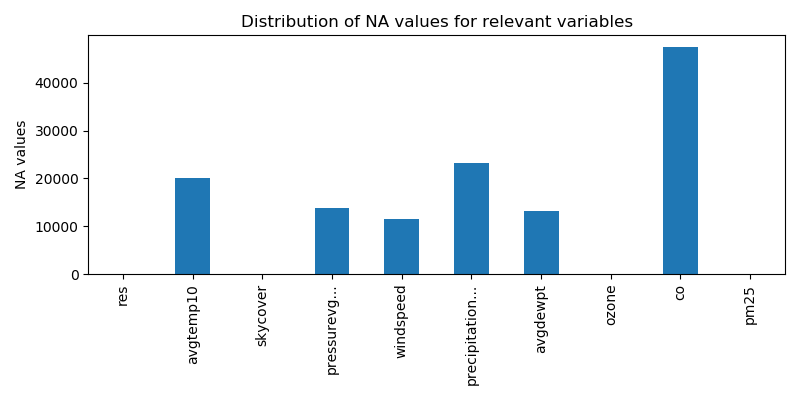
\includegraphics[scale=0.85]{plot_na_dist_of_n_cols_with_most_na.png}		
		}
		\end{center}
	
		\begin{center}
		\captionof{figure}{Yearly observation count} \label{tab:title} 
		{
		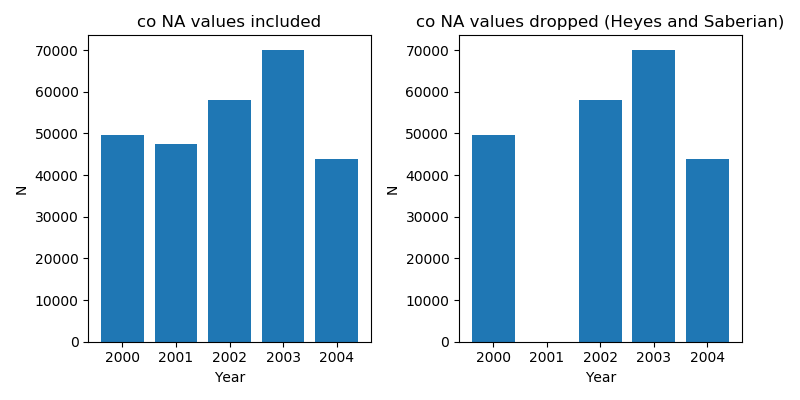
\includegraphics[scale=0.85]{double_plot_year_dist_with_and_whithout_co.png}	
		}
		\end{center}		
		
		
	\end{subappendices}	
	
	
	
	
	%%%%%%%%%%%%%%%%%%%%%%%%%%%%%%%%%%%%%%%%%%%%%%%%%%%%%%%%%%%%
	% References
	%%%%%%%%%%%%%%%%%%%%%%%%%%%%%%%%%%%%%%%%%%%%%%%%%%%%%%%%%%%%
	\newpage
	{\footnotesize 
		\bibliographystyle{apalike}
		\singlespacing
		\bibliography{manual_bibfile.bib}
	}
	
	
	%%%%%%%%%%%%%%%%%%%%%%%%%%%%%%%%%%%%%%%%%%%%%%%%%%%%%%%%%%%%
\end{document}